\documentclass[aspectratio=169,11pt]{beamer}

\usetheme{Madrid}
\usecolortheme{default}
\usefonttheme{professionalfonts}
\setbeamertemplate{navigation symbols}{}
\setbeamertemplate{blocks}[rounded][shadow=false]

\usepackage[T1]{fontenc}
\usepackage[utf8]{inputenc}
\usepackage{lmodern}
\usepackage{amsmath}
\usepackage{booktabs}
\usepackage{tabularx}
\usepackage{array}
\usepackage{graphicx}
\usepackage{tikz}
\usepackage{ragged2e}
\usepackage{xcolor}

\definecolor{AgroGreen}{HTML}{2F6B3B}
\definecolor{AgroLeaf}{HTML}{7FAE63}
\definecolor{AgroSoil}{HTML}{8C5A3C}
\definecolor{AgroCream}{HTML}{F7F3EA}
\definecolor{AgroInk}{HTML}{1E2A1F}
\definecolor{AgroGold}{HTML}{D9A441}

\setbeamercolor{normal text}{fg=AgroInk,bg=white}
\setbeamercolor{structure}{fg=AgroGreen}
\setbeamercolor{frametitle}{fg=white,bg=AgroGreen}
\setbeamercolor{title}{fg=white}
\setbeamercolor{subtitle}{fg=AgroCream}
\setbeamercolor{author}{fg=AgroCream}
\setbeamercolor{date}{fg=AgroCream}
\setbeamercolor{block title}{fg=white,bg=AgroGreen}
\setbeamercolor{block body}{fg=AgroInk,bg=AgroCream}
\setbeamercolor{itemize item}{fg=AgroGold}
\setbeamercolor{itemize subitem}{fg=AgroLeaf}

\setbeamerfont{title}{series=\bfseries,size=\Large}
\setbeamerfont{frametitle}{series=\bfseries,size=\large}

\newcommand{\accentline}{\textcolor{AgroGold}{\rule{\linewidth}{1.1pt}}}

\title{Agri MLLM}
\subtitle{A Multimodal Agricultural Assistant for Text, Image, and Audio Queries}
\author{M.\,Bourich \quad M.\,El Ansari \quad Y.\,Anouar}
\date{April 2026}

\begin{document}

{
\setbeamertemplate{background}{

\begin{tikzpicture}[remember picture,overlay]
\fill[AgroGreen] (current page.south west) rectangle (current page.north east);
\fill[AgroLeaf, opacity=0.18] (current page.north east) circle [radius=2.8cm];
\fill[AgroGold, opacity=0.10] (current page.south west) circle [radius=3.2cm];
\end{tikzpicture}
}
\begin{frame}[plain]
    \titlepage
    \vspace{-0.6em}
    
\end{frame}
}

\begin{frame}{Talk Roadmap}
\begin{itemize}
    \item Problem and product vision
    \item Platform experience and supported modalities
    \item Model architecture and training pipeline
    \item Datasets, results, and example output
    \item Limitations and next steps
\end{itemize}
\end{frame}

\begin{frame}{Problem We Are Solving}
\begin{block}{Core Need}
Farmers, students, and agronomy practitioners need quick crop-health guidance without always typing long technical descriptions.
\end{block}
\vspace{0.4em}
\begin{itemize}
    \item Disease recognition often depends on both \textbf{visual cues} and \textbf{domain knowledge}.
    \item Many users prefer different input modes depending on context:
    \begin{itemize}
        \item field image + typed question,
        \item text-only agronomy question,
        \item spoken question when hands are busy.
    \end{itemize}
    \item The goal is one assistant that can unify these entry points.
\end{itemize}
\end{frame}

\begin{frame}{Inspiration and Our Adaptation}
\begin{columns}[T]
    \column{0.48\textwidth}
    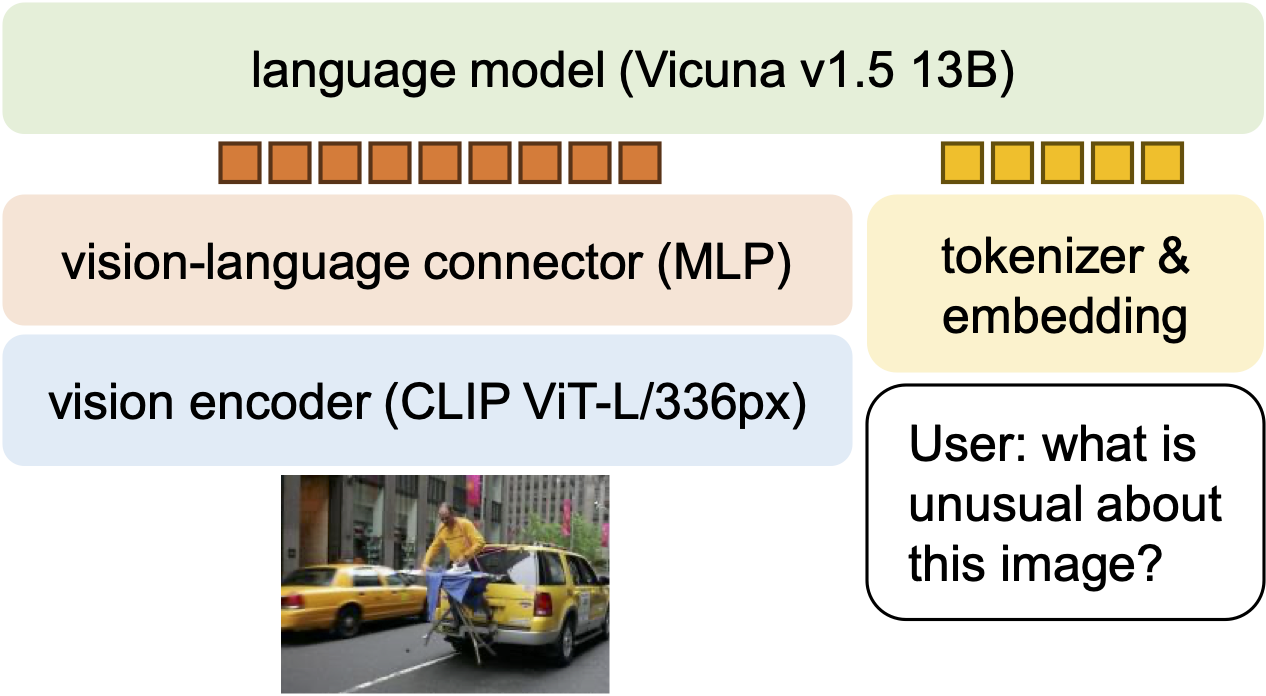
\includegraphics[width=\linewidth,height=0.62\textheight,keepaspectratio]{assets/llava15_architecture.png}
    \small
    \begin{block}{Inspired by LLaVA-1.5}
    \begin{itemize}
        \item CLIP vision encoder
        \item simple MLP vision-language connector
        \item efficient visual instruction tuning recipe
    \end{itemize}
    \end{block}
    \column{0.48\textwidth}


    \begin{block}{Adapted to our setting}
    \begin{itemize}
        \item domain goal: agriculture, not general vision chat
        \item domain data: KisanVaani + PlantVillage
        \item compute constraints: Qwen2.5-0.5B, LoRA, Colab T4
        \item design choice: keep all 256 spatial patches for leaf-level detail
    \end{itemize}
    \end{block}
\end{columns}
\vspace{1}
\tiny Inspired by \textit{Improved Baselines with Visual Instruction Tuning}; figure extracted from \texttt{papers/2310.03744v2.pdf}.

\end{frame}





\begin{frame}{Platform Vision}

    \begin{block}{A Multimodal ChatBot}
    \begin{itemize}
        \item \textbf{Image + text}: ``What disease is visible and how severe is it?''
        \item \textbf{Text only}: ``How much phosphorus per hectare should I apply to wheat?''
        \item \textbf{Audio only}: spoken agronomy question captured by the platform
        \item \textbf{PDF files}
    \end{itemize}
    \end{block}



\end{frame}

\begin{frame}{What the Repository Actually Implements}
\begin{itemize}
    \item \textbf{Base language model}: \texttt{Qwen/Qwen2.5-0.5B-Instruct}
    \item \textbf{Vision encoder}: \texttt{openai/clip-vit-large-patch14}
    \item \textbf{Alignment module}: a two-layer \textbf{MLP projector}
    \item \textbf{Adaptation}: agriculture LoRA + visual LoRA
    \item \textbf{Training environment}: Google Colab T4 GPU
    \item \textbf{Deployment}: Streamlit frontend + FastAPI inference server
\end{itemize}
\end{frame}

\begin{frame}{End-to-End System Pipeline}
\begin{center}
\resizebox{0.95\linewidth}{!}{%
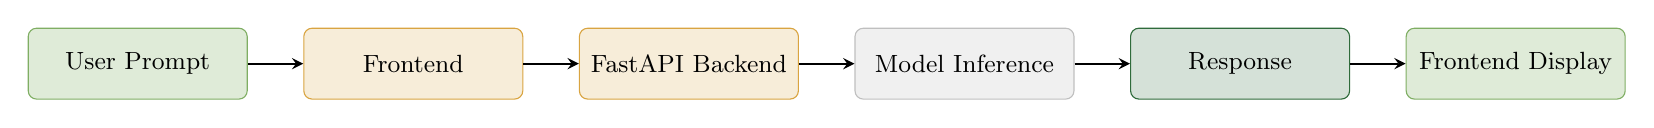
\begin{tikzpicture}[
    every node/.style={font=\small},
    box/.style={draw, rounded corners=3pt, align=center,
                text width=2.5cm, minimum height=0.9cm,
                inner sep=4pt},
    teal/.style  ={box, fill=AgroLeaf!25,  draw=AgroLeaf},
    purp/.style  ={box, fill=AgroGold!20,  draw=AgroGold},
    grayb/.style ={box, fill=gray!12,      draw=gray!50},
    greenb/.style={box, fill=AgroGreen!20, draw=AgroGreen},
    arr/.style={->, thick, >=stealth},
]

%% Nodes (single row)
\node[teal]   (user)      at (0,0)   {User Prompt};
\node[purp]   (frontend)  at (3.5,0) {Frontend};
\node[purp]   (api)       at (7,0)   {FastAPI Backend};
\node[grayb]  (model)     at (10.5,0){Model Inference};
\node[greenb] (resp)      at (14,0)  {Response};
\node[teal]   (display)   at (17.5,0){Frontend Display};

%% Arrows
\draw[arr] (user) -- (frontend);
\draw[arr] (frontend) -- (api);
\draw[arr] (api) -- (model);
\draw[arr] (model) -- (resp);
\draw[arr] (resp) -- (display);

\end{tikzpicture}
}%
\end{center}
\end{frame}

\begin{frame}{The Actual Model: From Input to Output}
\begin{center}
\resizebox{0.95\linewidth}{!}{%
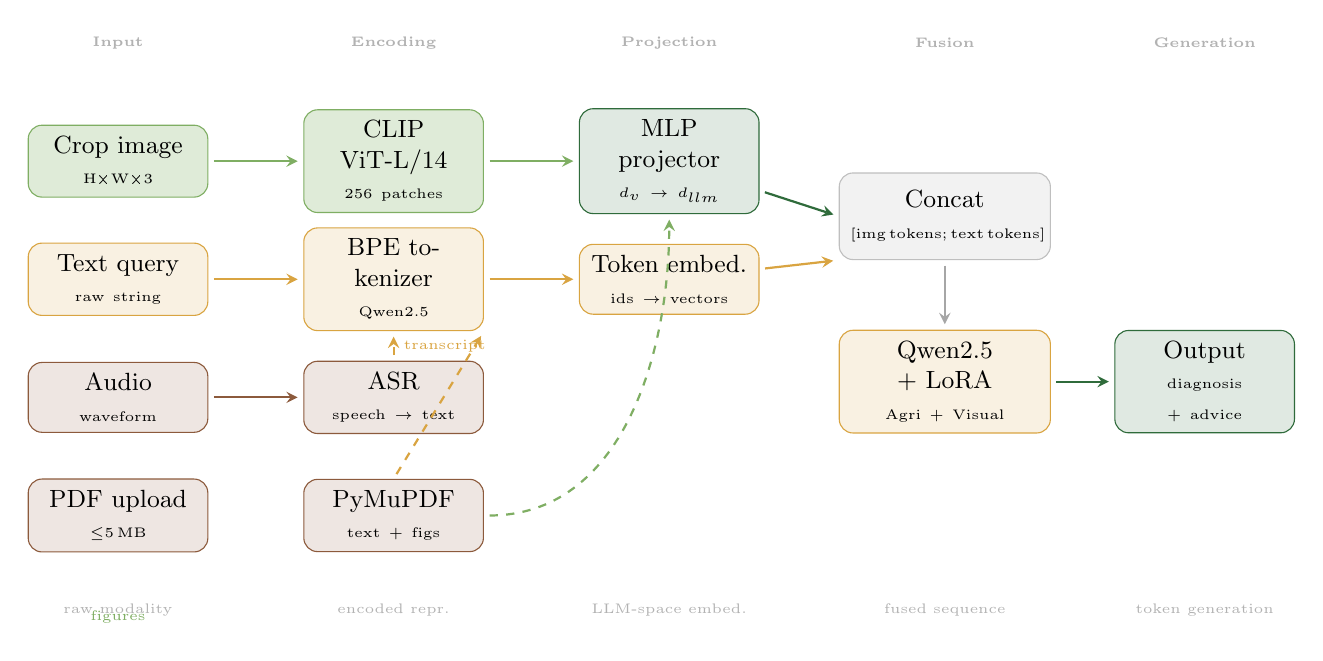
\begin{tikzpicture}[
  every node/.style={font=\small},
  box/.style={draw, rounded corners=5pt, align=center,
              text width=2.0cm, minimum height=0.85cm, inner sep=4pt},
  teal/.style ={box, fill=AgroLeaf!25,  draw=AgroLeaf},
  purp/.style ={box, fill=AgroGold!15,  draw=AgroGold},
  green/.style={box, fill=AgroGreen!15, draw=AgroGreen},
  gray/.style ={box, fill=gray!10,      draw=gray!50},
  amber/.style={box, fill=AgroSoil!15,  draw=AgroSoil},
  stage/.style={font=\tiny\bfseries, text=gray!60},
  arr/.style={->, thick, >=stealth, shorten >=2pt, shorten <=2pt},
]

%% ── Stage headers ────────────────────────────
\node[stage] at (0,    7.5) {Input};
\node[stage] at (3.5,  7.5) {Encoding};
\node[stage] at (7.0,  7.5) {Projection};
\node[stage] at (10.5, 7.5) {Fusion};
\node[stage] at (13.8, 7.5) {Generation};

%% ── Row 1: Image ─────────────────────────────
\node[teal]  at (0,   6.0) (img)  {Crop image\\\tiny H×W×3};
\node[teal]  at (3.5, 6.0) (clip) {CLIP ViT-L/14\\\tiny 256 patches};
\node[green] at (7.0, 6.0) (mlp)  {MLP projector\\\tiny $d_v \to d_{llm}$};

%% ── Row 2: Text ──────────────────────────────
\node[purp]  at (0,   4.5) (txt)  {Text query\\\tiny raw string};
\node[purp]  at (3.5, 4.5) (btok) {BPE tokenizer\\\tiny Qwen2.5};
\node[purp]  at (7.0, 4.5) (emb)  {Token embed.\\\tiny ids $\to$ vectors};

%% ── Row 3: Audio (merges into text row) ───────
\node[amber] at (0,   3.0) (aud)  {Audio\\\tiny waveform};
\node[amber] at (3.5, 3.0) (asr2) {ASR\\\tiny speech $\to$ text};

%% ── Row 4: PDF ───────────────────────────────
\node[amber] at (0,   1.5) (pdf2) {PDF upload\\\tiny $\leq$5\,MB};
\node[amber] at (3.5, 1.5) (mup2) {PyMuPDF\\\tiny text + figs};

%% ── Fusion node ──────────────────────────────
\node[gray, text width=2.4cm, minimum height=1.1cm]
             at (10.5, 5.3) (cat)  {Concat\\
             \tiny [img\,tokens;\,text\,tokens]};

%% ── LLM + output ─────────────────────────────
\node[purp, text width=2.4cm]
             at (10.5, 3.2) (llm2) {Qwen2.5 + LoRA\\\tiny Agri + Visual};
\node[green] at (13.8, 3.2) (out2) {Output\\\tiny diagnosis + advice};

%% ── Arrows row 1 ─────────────────────────────
\draw[arr, AgroLeaf]  (img)  -- (clip);
\draw[arr, AgroLeaf]  (clip) -- (mlp);
\draw[arr, AgroGreen] (mlp)  -- (cat.west);

%% ── Arrows row 2 ─────────────────────────────
\draw[arr, AgroGold]  (txt)  -- (btok);
\draw[arr, AgroGold]  (btok) -- (emb);
\draw[arr, AgroGold]  (emb)  -- (cat.south west);

%% ── Audio → tokenizer ────────────────────────
\draw[arr, AgroSoil]  (aud)  -- (asr2);
\draw[arr, AgroGold, dashed]  (asr2.north) --
    node[right, font=\tiny, AgroGold]{transcript} (btok.south);

%% ── PDF text → tokenizer; figures → projector ─
\draw[arr, AgroGold, dashed]  (mup2.north) -- (btok.south east);
\draw[arr, AgroLeaf, dashed]  (mup2.east)
    to[out=0, in=270] (mlp.south)
    node[near start, above, font=\tiny, AgroLeaf]{figures};

%% ── Fusion → LLM → output ────────────────────
\draw[arr, gray!70]   (cat)  -- (llm2);
\draw[arr, AgroGreen] (llm2) -- (out2);

%% ── Data-type annotations ────────────────────
\node[font=\tiny, gray!60, align=center] at (0,   0.3)
    {raw modality};
\node[font=\tiny, gray!60, align=center] at (3.5, 0.3)
    {encoded repr.};
\node[font=\tiny, gray!60, align=center] at (7.0, 0.3)
    {LLM-space embed.};
\node[font=\tiny, gray!60, align=center] at (10.5,0.3)
    {fused sequence};
\node[font=\tiny, gray!60, align=center] at (13.8,0.3)
    {token generation};

\end{tikzpicture}
}%
\end{center}
\end{frame}

\begin{frame}{Training Pipeline in Three Steps}
\begin{enumerate}
    \item \textbf{Stage 0 Text-only domain adaptation}
    \begin{itemize}
        \item Fine-tune a LoRA on agricultural QA text.
    \end{itemize}
    \item \textbf{Stage 1 visual alignment}
    \begin{itemize}
        \item Freeze ViT and LLM.
        \item Train only the projector on image-caption pairs.
    \end{itemize}
    \item \textbf{Stage 2 multimodal adaptation}
    \begin{itemize}
        \item Keep ViT frozen.
        \item Train projector + new visual LoRA on VQA triplets.
    \end{itemize}
\end{enumerate}
\vspace{0.4em}
\begin{block}{Why this works}
The pipeline first teaches the model agricultural language, then teaches image tokens to ``speak'' the LLM embedding space, then tunes multimodal reasoning.
\end{block}
\end{frame}

\begin{frame}{Stage 0: Prepare the Agriculture-Aware LLM}
\begin{tabular}{ll}
\toprule
\textbf{Component} & \textbf{Details} \\
\midrule
Train  & LoRA on base LLM \\
Data   & Agriculture text corpus: KisanVaani/agriculture-qa-english-only \\
Loss   & Causal LM (next token prediction) \\
Result & LLM that knows plant diseases, agronomic terminology \\
\bottomrule
\end{tabular}
\vspace{0.4em}
\begin{itemize}
    \item Source in code: \texttt{KisanVaani/agriculture-qa-english-only}
    \item Processed rows in logs: \textbf{22,574 usable}; training JSONL subset: \textbf{8,000}
    \item Stage 0 setup: \textbf{450 max steps}, effective batch size \textbf{16}
\end{itemize}
\end{frame}

\begin{frame}{Stage 0 Plot: LLM Fine-Tuning}
\begin{columns}[T]
    \column{0.62\textwidth}
    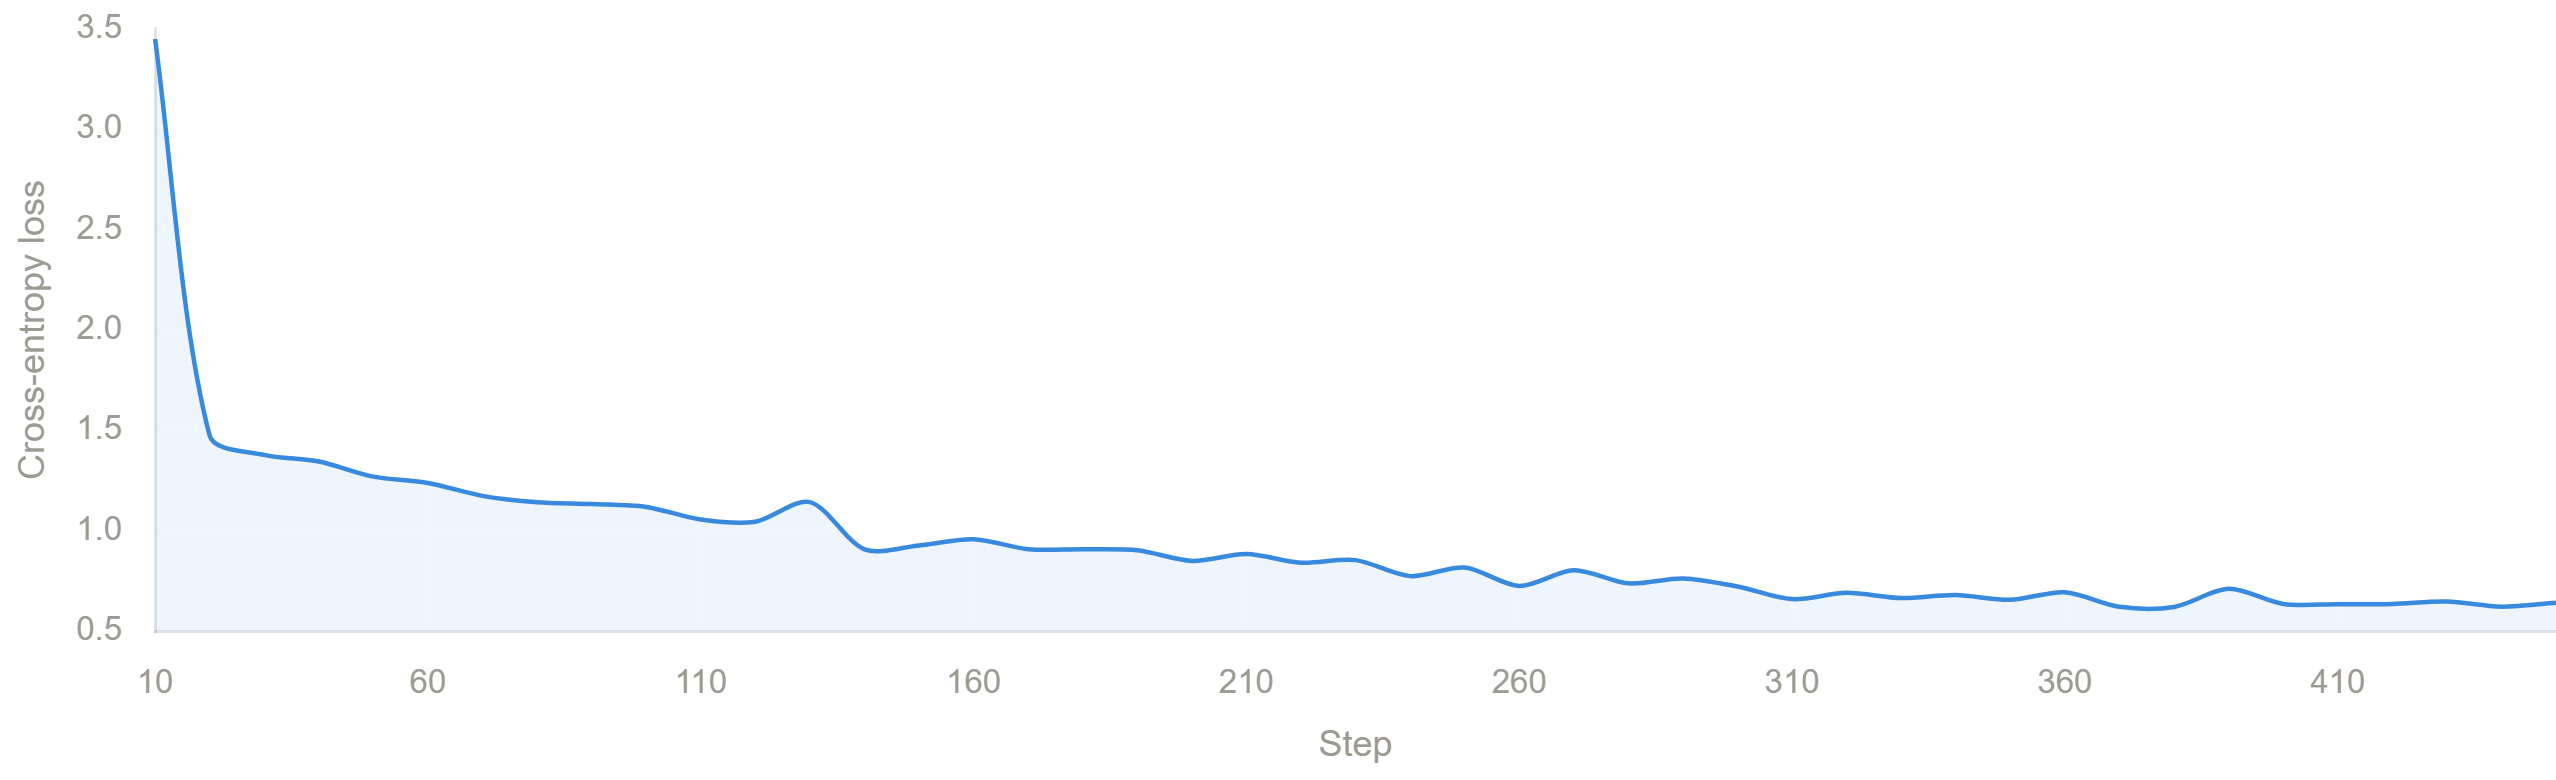
\includegraphics[width=\linewidth,height=0.72\textheight,keepaspectratio]{plots/LLM fine-tuning loss curve.png}

    \column{0.34\textwidth}
    \small
    \begin{block}{What changed}
    \begin{itemize}
        \item LoRA trained on \textbf{8,000} agricultural QA samples
        \item Sharp early drop, then steady convergence
        \item Final logged train loss: \textbf{0.9349}
    \end{itemize}
    \end{block}
%%    \begin{block}{Reading}
 %%   The HTML report notes the curve falls fast in the first 100 steps, then continues decreasing through the 450-step run.
 %%   \end{block}
\end{columns}
\end{frame}

\begin{frame}{Stage 1: Train the Visual Projector}
\begin{tabular}{ll}
\toprule
\textbf{Component} & \textbf{Details} \\
\midrule
Freeze  & ViT + LLM \\
Train   & MLP projector only \\
Data    & (image, caption) pairs from disease dataset (PlantVillage) \\
Loss    & Causal LM on captions given image tokens \\
Result  & Projector that speaks the LLM's embedding language \\
Purpose & Alignment stage --- teach image tokens to look like text tokens \\
\bottomrule
\end{tabular}
\end{frame}
\begin{frame}{Stage 1 Plot: Caption Alignment}
\begin{columns}[T]
    \column{0.62\textwidth}
    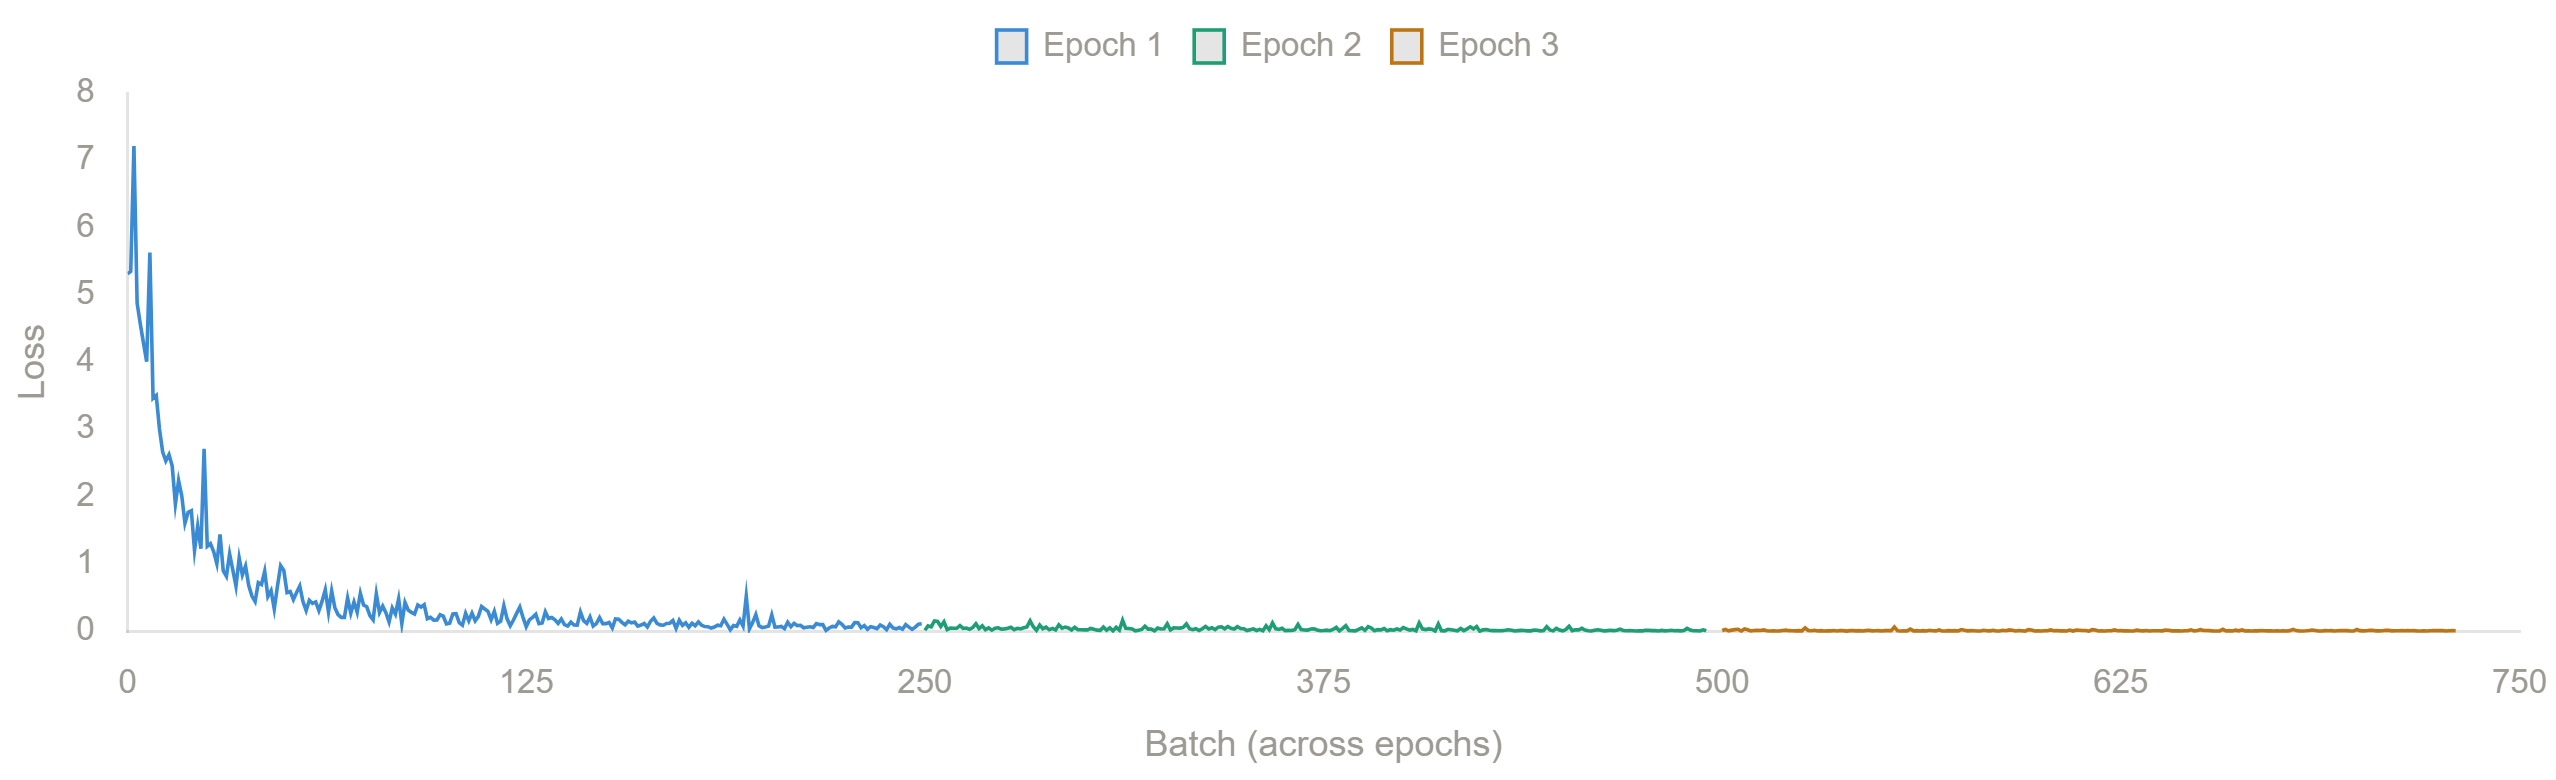
\includegraphics[width=\linewidth,height=0.72\textheight,keepaspectratio]{plots/Projector loss curves (caption alignment).png}

    \column{0.34\textwidth}
    \small

    \begin{block}{Interpretation}
    This is the cleanest convergence phase in the pipeline and shows that the projector successfully learns the vision-to-language bridge.
    \end{block}
\end{columns}
\end{frame}

\begin{frame}{Stage 2: Fine-tune End-to-End with LoRA}
\begin{tabular}{ll}
\toprule
\textbf{Component} & \textbf{Details} \\
\midrule
Freeze & ViT \\
Train  & MLP projector + new LoRA layers in LLM \\
Data   & (image, question, answer) triplets --- disease VQA (PlantVillage) \\
Loss   & Causal LM on answers \\
Result & Full multimodal agriculture assistant \\
\bottomrule
\end{tabular}
\vspace{0.4em}
\begin{itemize}
    \item Stage 2 set in logs: \textbf{1,000} generated VQA triplets from PlantVillage
    \item \textbf{4} QA pairs sampled per image from 5 templates
\end{itemize}
\end{frame}
\begin{frame}{Stage 2 Plot: VQA Alignment}
\begin{columns}[T]
    \column{0.62\textwidth}
    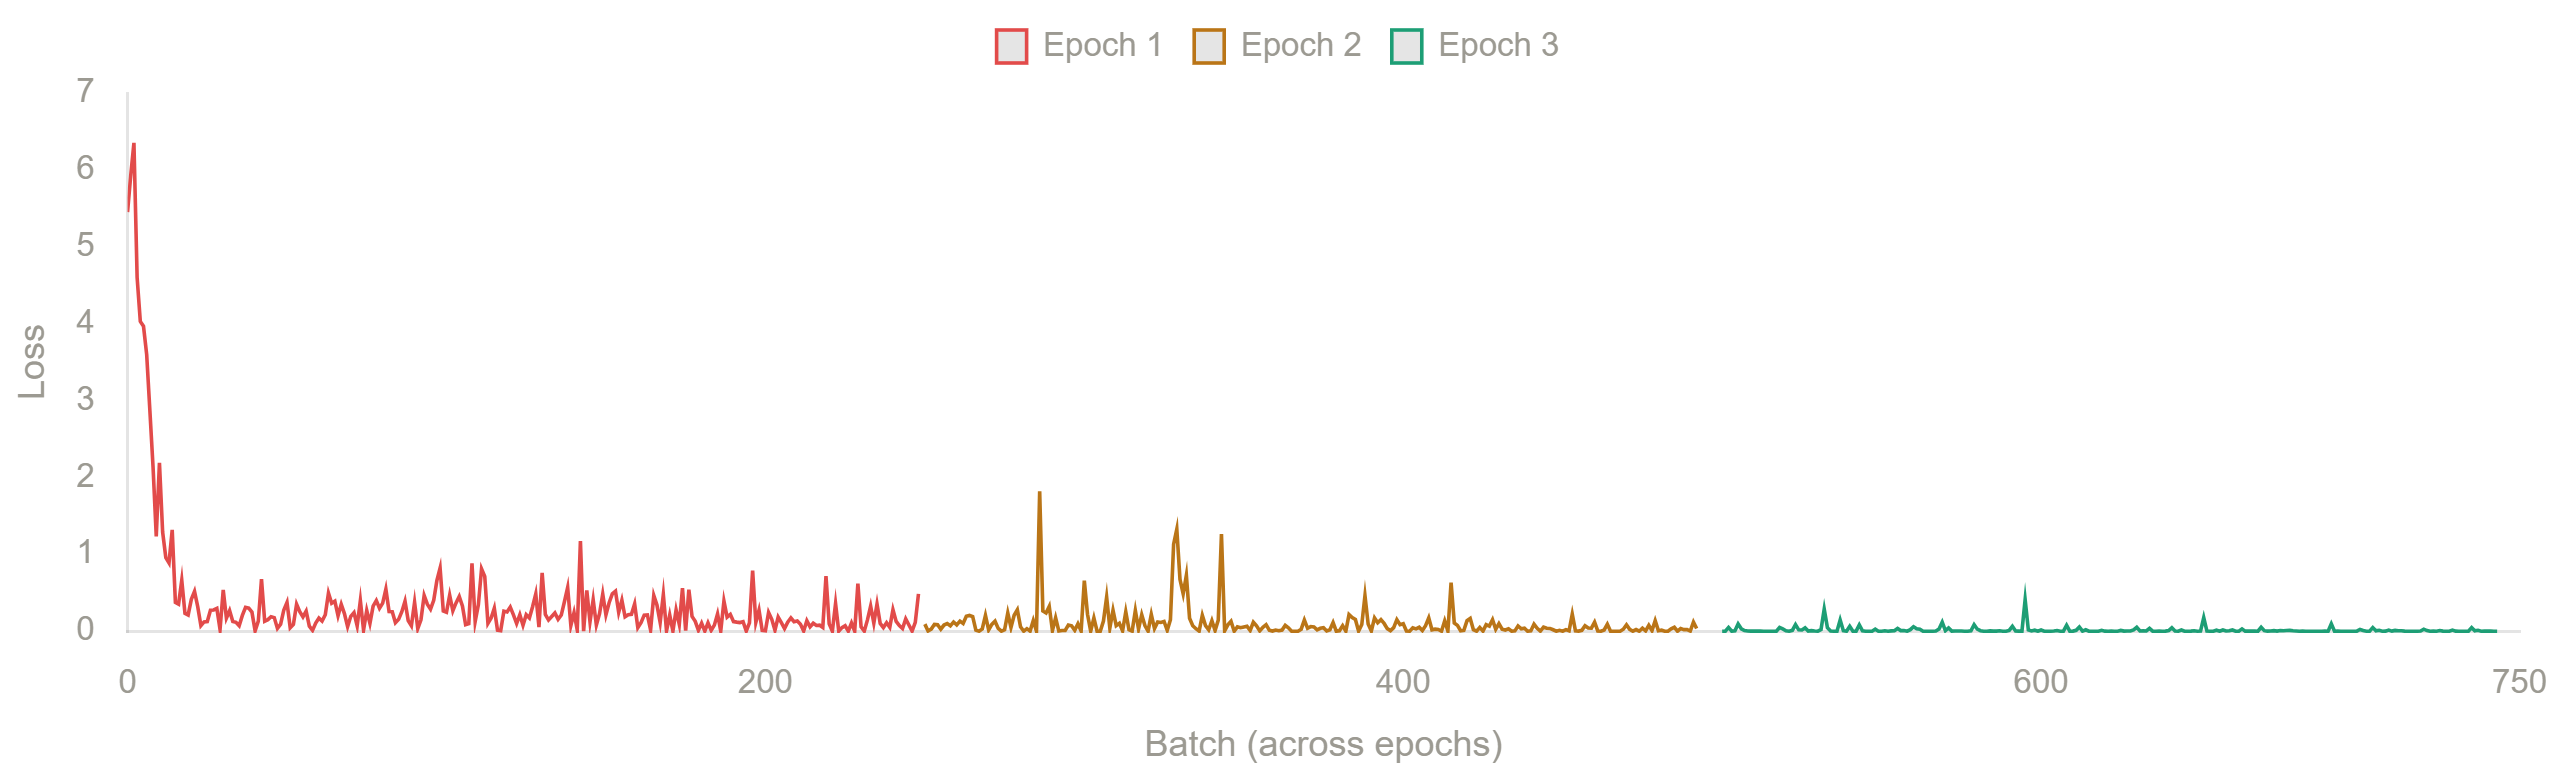
\includegraphics[width=\linewidth,height=0.72\textheight,keepaspectratio]{plots/Projectorlosscurves_(VQA alignment).png}

    \column{0.34\textwidth}
    \small

    \begin{block}{Interpretation}
    The first epoch is noisier because VQA is harder than captioning, but the run still converges cleanly by epoch 3.
    \end{block}
\end{columns}
\end{frame}

\begin{frame}{Training Snapshot}
\small
\begin{center}
\begin{tabularx}{\linewidth}{lccc}
\toprule
\textbf{Phase} & \textbf{Epoch / Run} & \textbf{Metric} & \textbf{Value} \\
\midrule
Text LoRA & final run & train loss & 0.9349 \\
Projector Stage 1 & epoch 1 & avg loss & 0.5500 \\
Projector Stage 1 & epoch 2 & avg loss & 0.0347 \\
Projector Stage 1 & epoch 3 & avg loss & 0.0090 \\
Stage 2 multimodal & epoch 1 & avg loss & 0.3996 \\
Stage 2 multimodal & epoch 2 & avg loss & 0.0994 \\
Stage 2 multimodal & epoch 3 & avg loss & 0.0141 \\
\bottomrule
\end{tabularx}
\end{center}
\vspace{0.4em}
\begin{itemize}
    \item Report summary: \textbf{8.8M trainable parameters}, about \textbf{1.75\%} of a 502M-parameter model.
    \item Stage 0 runtime reported: \textbf{1007 seconds} with about \textbf{7.15 samples/s}.
\end{itemize}
\end{frame}

\begin{frame}{Audio Modality Integration}

\begin{columns}[T]
    \column{0.58\textwidth}
    \begin{figure}
    \centering
    \resizebox{\linewidth}{!}{%
    \begin{tikzpicture}[
        every node/.style={font=\small},
        box/.style={draw, rounded corners=3pt, align=center,
                    text width=1.8cm, minimum height=0.75cm,
                    inner sep=4pt},
        teal/.style  ={box, fill=AgroLeaf!25,  draw=AgroLeaf},
        purp/.style  ={box, fill=AgroGold!20,  draw=AgroGold},
        grayb/.style ={box, fill=gray!12,      draw=gray!50},
        greenb/.style={box, fill=AgroGreen!20, draw=AgroGreen},
        arr/.style={->, thick, >=stealth, shorten >=2pt, shorten <=2pt},
    ]

    %% ── Column 1: inputs (x=0) ──────────────────────────────────
    \node[teal]  at (0,  1.5) (audio) {Audio input\\\tiny farmer speaks};
    \node[purp]  at (0,  0.0) (text)  {Text input\\\tiny typed question};

    %% ── Column 2: processing (x=3) ─────────────────────────────
    \node[teal]  at (3,  1.5) (asr)  {ASR module\\\tiny speech-to-text};
    \node[purp]  at (3,  0.0) (tok)  {Tokenizer\\\tiny Qwen2.5 BPE};

    %% ── Column 3: output (x=6) ──────────────────────────────────
    \node[grayb]  at (6,  0.0) (llm)  {LLM + LoRA\\\tiny Qwen2.5 adapters};
    \node[greenb] at (6,  1.5) (out)  {Response\\\tiny diagnosis/advice};

    %% ── Arrows ──────────────────────────────────────────────────
    \draw[arr] (audio) -- (asr);
    \draw[arr] (text)  -- (tok);

    %% ASR drops down to tokenizer
    \draw[arr, AgroGold] (asr) -- (tok)
        node[midway, right, font=\tiny\itshape,
             text=AgroGold, xshift=1pt] {transcript};

    \draw[arr] (tok) -- (llm);
    \draw[arr] (llm) -- (out);

    %% ── Platform boundary dashed box ────────────────────────────
    \begin{scope}[on background layer]
        \node[draw=AgroLeaf, dashed, rounded corners=6pt,
              fit=(audio)(asr)(tok),
              inner sep=7pt,
              label={[font=\tiny, color=AgroLeaf]above:platform layer}] {};
    \end{scope}

    \end{tikzpicture}
    }%
    \caption{\footnotesize Audio follows the same inference path as typed text once transcribed.}
    \end{figure}

    \column{0.39\textwidth}
    \vspace{0.4em}
    \begin{block}{Key points}
    \begin{itemize}
        \item \textbf{ASR} lives in the platform layer not inside the model
        \item Transcript enters the \textbf{same tokenizer} as typed text
        \item Agriculture LoRA handles both typed and spoken queries unchanged
        \item Audio is a new \textbf{entry interface}, not a new reasoning pathway
    \end{itemize}
    \end{block}

\end{columns}
\end{frame}
\begin{frame}{PDF Modality Integration}
\begin{columns}[T]
    \column{0.58\textwidth}
    \vspace{0.4em}
    \begin{center}
    \resizebox{\linewidth}{!}{%
    \begin{tikzpicture}[
        every node/.style={font=\small},
        box/.style={draw, rounded corners=3pt, align=center,
                    text width=2.0cm, minimum height=0.75cm,
                    inner sep=4pt},
        teal/.style  ={box, fill=AgroLeaf!25,  draw=AgroLeaf},
        purp/.style  ={box, fill=AgroGold!20,  draw=AgroGold},
        amber/.style ={box, fill=AgroSoil!20,  draw=AgroSoil},
        grayb/.style ={box, fill=gray!12,      draw=gray!50},
        greenb/.style={box, fill=AgroGreen!20, draw=AgroGreen},
        arr/.style={->, thick, >=stealth, shorten >=2pt, shorten <=2pt},
    ]

    %% ── Column 1 (x=0) ──────────────────────────────────────────
    \node[teal]  at (0,  1.5) (pdf)   {PDF upload\\\tiny max 5\,MB};
    \node[purp]  at (0,  0.0) (check) {Size check\\\tiny PyMuPDF};

    %% ── Column 2: two branches (x=3) ────────────────────────────
    \node[purp]  at (3,  2.6) (text)  {Text extraction\\\tiny 8 pages · 2k chars};
    \node[amber] at (3,  0.0) (fig)   {Figure extraction\\\tiny first 2 figures};

    %% ── Column 3: processing (x=6) ──────────────────────────────
    \node[purp]  at (6,  2.6) (trunc) {Token cap\\\tiny 1{,}200 tokens};
    \node[amber] at (6,  0.0) (enc)   {Vision encoder\\\tiny $\geq$64$\times$64 px};

    %% ── Column 4: fusion + output (x=9) ─────────────────────────
    \node[grayb]  at (9,  1.5) (fuse) {Fusion\\\tiny text + figures};
    \node[greenb] at (9,  3.2) (out)  {LLM answer\\\tiny multimodal};

    %% ── Arrows ──────────────────────────────────────────────────
    \draw[arr] (pdf)   -- (check);
    %% check splits into two branches
    \draw[arr] (check) -- (text)
        node[midway, left, font=\tiny, xshift=-2pt] {};
    \draw[arr] (check) -- (fig);

    \draw[arr] (text)  -- (trunc);
    \draw[arr] (fig)   -- (enc)
        node[midway, above, font=\tiny\itshape,
             text=AgroSoil] {if multimodal};

    \draw[arr] (trunc) -- (fuse);
    \draw[arr] (enc)   -- (fuse);
    \draw[arr] (fuse)  -- (out);

    %% ── Platform boundary dashed box ────────────────────────────
    \begin{scope}[on background layer]
        \node[draw=AgroLeaf, dashed, rounded corners=6pt,
              fit=(pdf)(check)(text)(fig)(trunc)(enc),
              inner sep=7pt,
              label={[font=\tiny, color=AgroLeaf]above:platform layer}] {};
    \end{scope}

    \end{tikzpicture}
    }%
    \end{center}

    \column{0.39\textwidth}
    \vspace{0.4em}
    \begin{block}{Key points}
    \begin{itemize}
        \item PDFs capped at \textbf{5\,MB}; parsed with PyMuPDF
        \item Text: first \textbf{8 pages}, 2{,}000 chars/page, \textbf{1{,}200 token} cap
        \item Figures: first \textbf{2 figures}, images $<$64$\times$64 px ignored
        \item Figures encoded by the \textbf{vision encoder} and passed through the PDF figure projector
        \item Text and figure tokens \textbf{fused} with the user question before the LLM
    \end{itemize}
    \end{block}

\end{columns}
\end{frame}
\begin{frame}{Demo - Text Only}
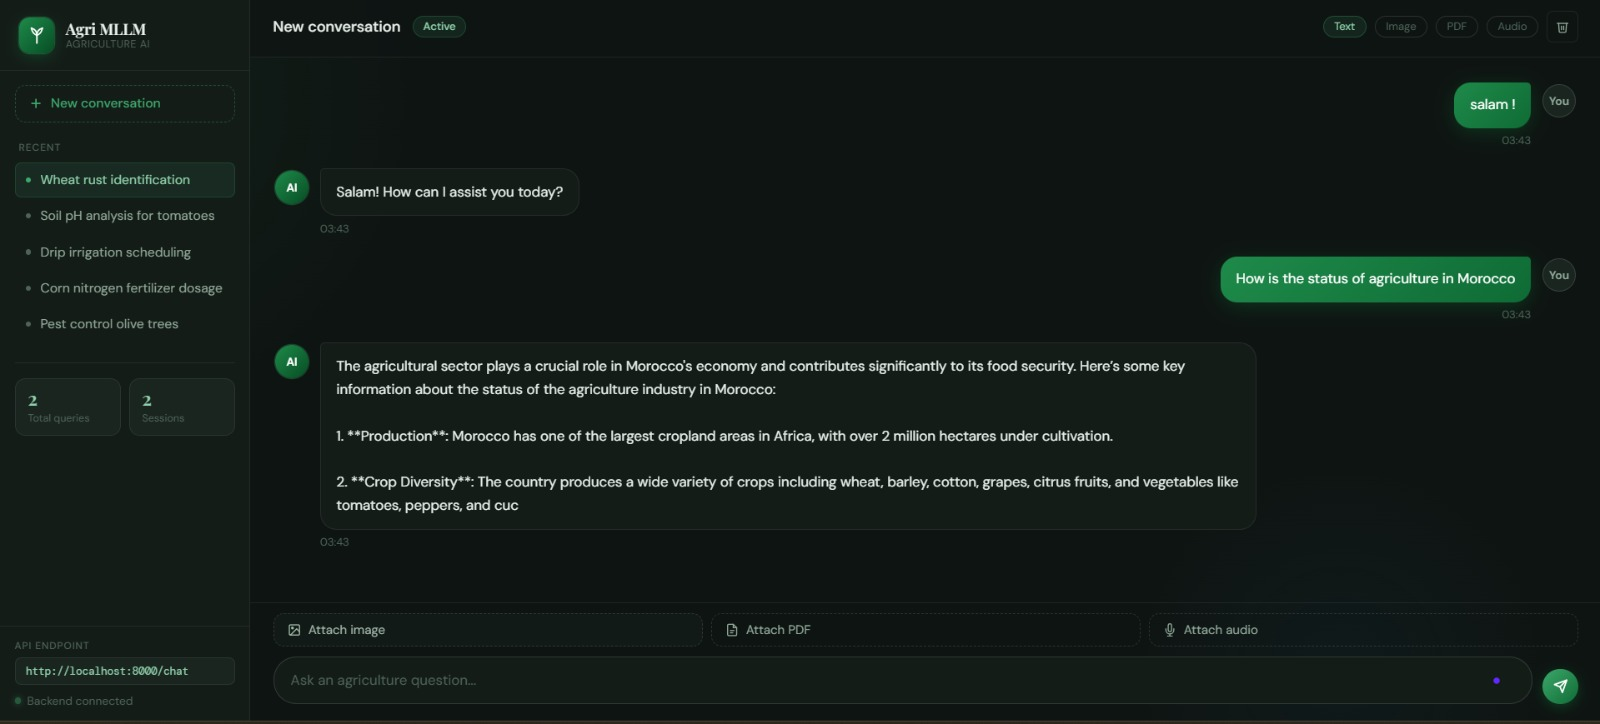
\includegraphics[width=\textwidth]{demo/txt.png}
\end{frame}
\begin{frame}{Demo - Image \& Text}
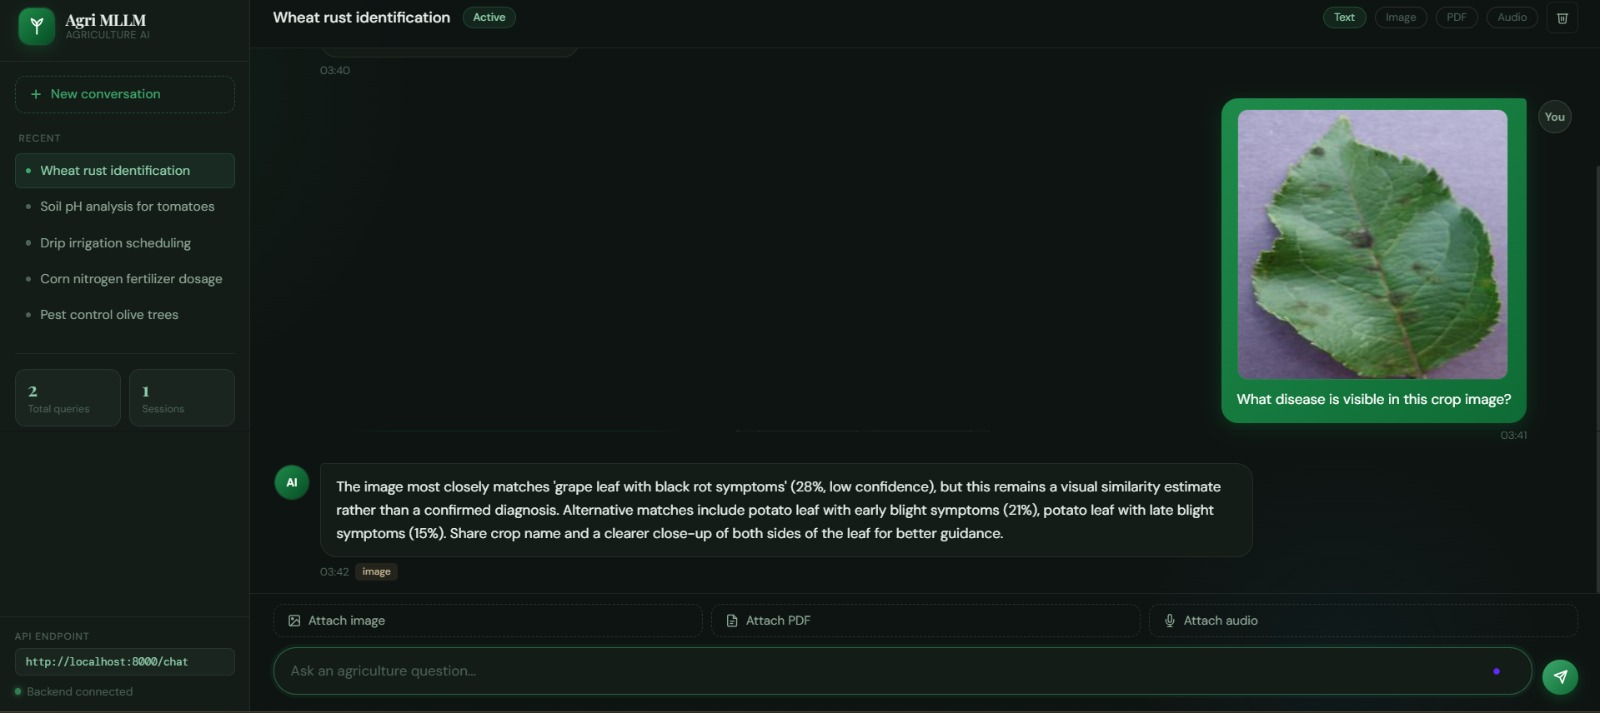
\includegraphics[width=\textwidth]{demo/img-txt0.png}

\end{frame}
\begin{frame}{Demo - Image \& Text}
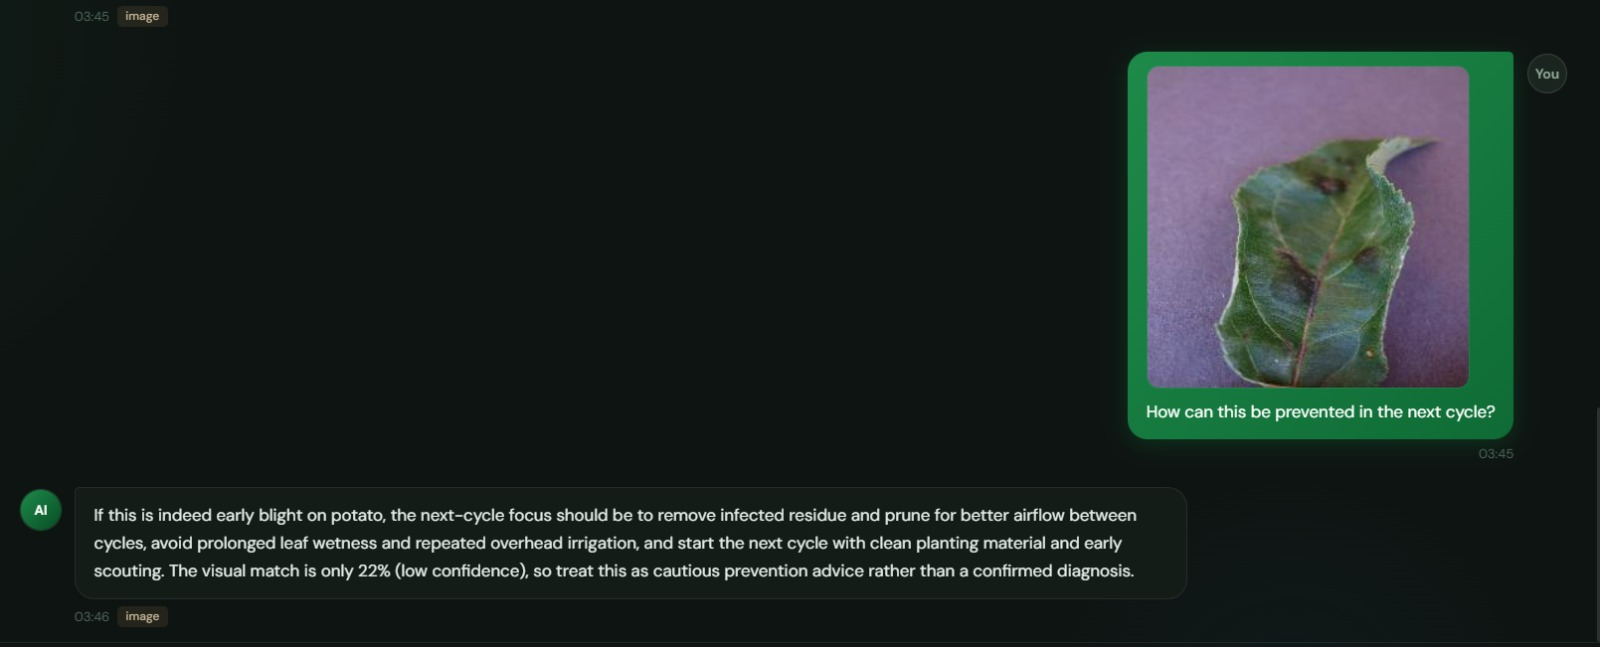
\includegraphics[width=\textwidth]{demo/img-txt1.png}
\end{frame}
\begin{frame}{Demo - Audio}
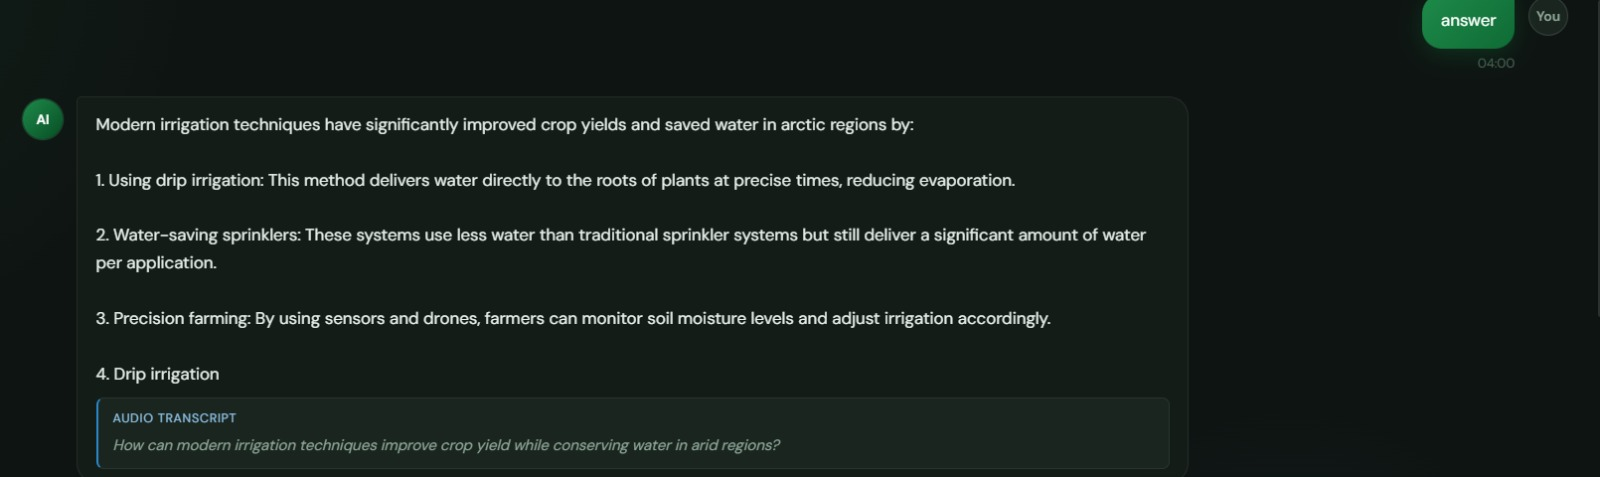
\includegraphics[width=\textwidth]{demo/audio.png}
\end{frame}
\begin{frame}{Demo - PDF File}
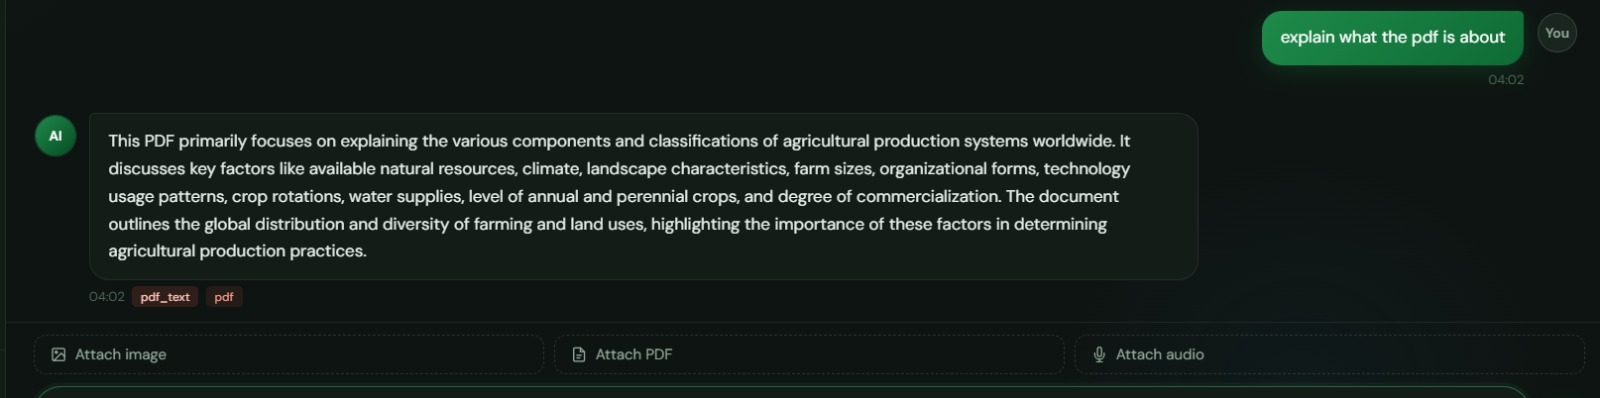
\includegraphics[width=\textwidth]{demo/pdf.png}
\end{frame}


\begin{frame}{Current Limitations}
\begin{itemize}
    \item Multimodal supervision is partly template-generated, so linguistic diversity is limited.
    \item PlantVillage is curated and clean; field images in real farms may be harder.
    \item Stage 0 stops when the loss is at about \textbf{0.9}, so the language adapter has not yet fully covered the full text dataset.
    

\end{itemize}
\end{frame}

\begin{frame}{Next Steps}
\begin{enumerate}
    \item Connect live ASR to the deployed frontend for real spoken queries.
    \item Increase Stage 0 training beyond 450 steps and add validation-based early stopping.
    \item Validate on real field images beyond PlantVillage.
    \item Add multilingual prompts and speech support.
    \item Replace template-generated captions and VQA pairs with expert-reviewed supervision.
    \item Consider a larger backbone such as \texttt{Qwen2.5-1.5B} for stronger reasoning.
\end{enumerate}
\end{frame}

\begin{frame}{Takeaway}
\begin{block}{Final Message}
Agri MLLM is a strong prototype of a \textbf{multimodal agricultural assistant}:
\begin{itemize}
    \item trained first on agricultural text knowledge,
    \item aligned to \textbf{PlantVillage} crop-disease images,
    \item and presented as a platform that supports \textbf{text}, \textbf{image + text}, and \textbf{audio} interaction.
\end{itemize}
\end{block}
\vspace{0.5em}
\centering
\Large\textcolor{AgroGreen}{One assistant, multiple field-friendly ways to ask for help.}
\end{frame}
\begin{frame}{References}
\begin{itemize}
    \item Liu, H., Li, C., Li, Y., \& Lee, Y. J. (2024).  
    \textit{Improved Baselines with Visual Instruction Tuning}.  
    arXiv:2310.03744.  
    \url{https://arxiv.org/abs/2310.03744}
    
    \item Code repository:  
    \url{https://github.com/Uness10/HopefullyItWorks}
    \item Course Lectures
\end{itemize}
\end{frame}

\end{document}